\newpage
\section{Functional requirements}

The system contains a login function for both caseworkers and applicants. Caseworkers login to the system through an employee portal, while applicants login to the system using NemId. The system validates eligible applicants through NemId.

\vspace{2mm}

Once the applicant is logged in, they are presented with a form through which they submit relevant information. The form contains text input fields and fields through which additional documentation can be attached to the case as pdf files.

\vspace{2mm}

The system assigns submitted cases to available caseworkers at random. Processed cases are archived and saved in an immutable state. Cases are annotated based on their state, i.e. ongoing, archived or on hold. Cases from the same citizen are also annotated in order to detect possible duplicates.

\vspace{2mm}

Once logged in, the caseworker is presented with their assigned cases, as well as a way to search all archived cases. More specifically, the caseworker cannot see ongoing cases not assigned to them, however all archived cases are search-able no matter the assigned caseworker. Caseworkers have access to all data submitted in the cases by the applicant. While processing a case, the caseworker can approve or reject cases. If the case is approved, the system calculates the "loss of earnings" benefits based on the data contained in the case and the current applicable laws. The system informs the applicant of the final decision, containing the benefits calculations if approved, through an e-mail.

\vspace{2mm}

A caseworker can set a case on hold if the documentation is insufficient. In such a case, the cases state must be changed to on hold and the system sends an e-mail to the applicant informing them of the cases state. The caseworker is able to write the message contained in the e-mail. The applicant is able to access the case form through a link in the e-mail, where the applicant can submit the missing information. The caseworker can afterwards reprocess the case and either reject or approve the case.

\vspace{2mm}

A duplicate cases are annotated and they are clearly presented for the caseworker as such. The caseworker can confirm a case to be a duplicate or   In case the System annotated a case as a possible duplicate and the caseworker decides this to be true, then the case state must be changed to rejected.

\vspace{2mm}

A caseworker can be assigned a supervisor role, giving them additional functions. A supervisor is able to see all ongoing and archived cases, as well as which caseworkers has been assigned to which case and the cases current state.
\newpage
\begin{figure}[htb!]
	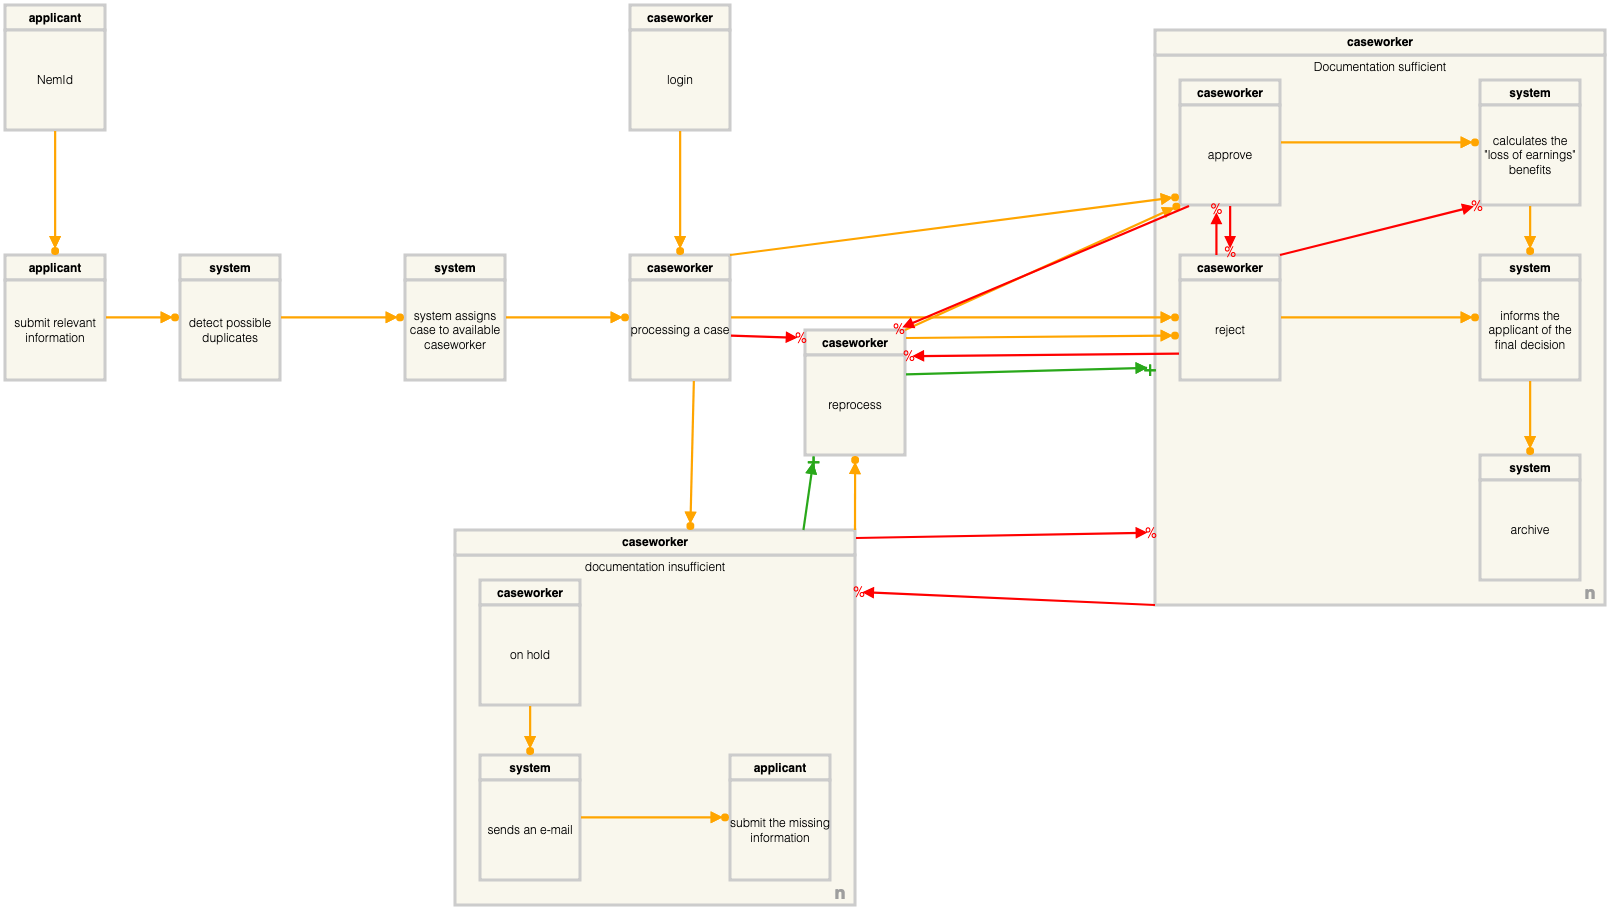
\includegraphics[width=\textwidth]{dcrgraph/dcrgraph.png}
	\caption{DCR graph}
\end{figure}

\newpage
\begin{figure}[htb!]
    \centering
    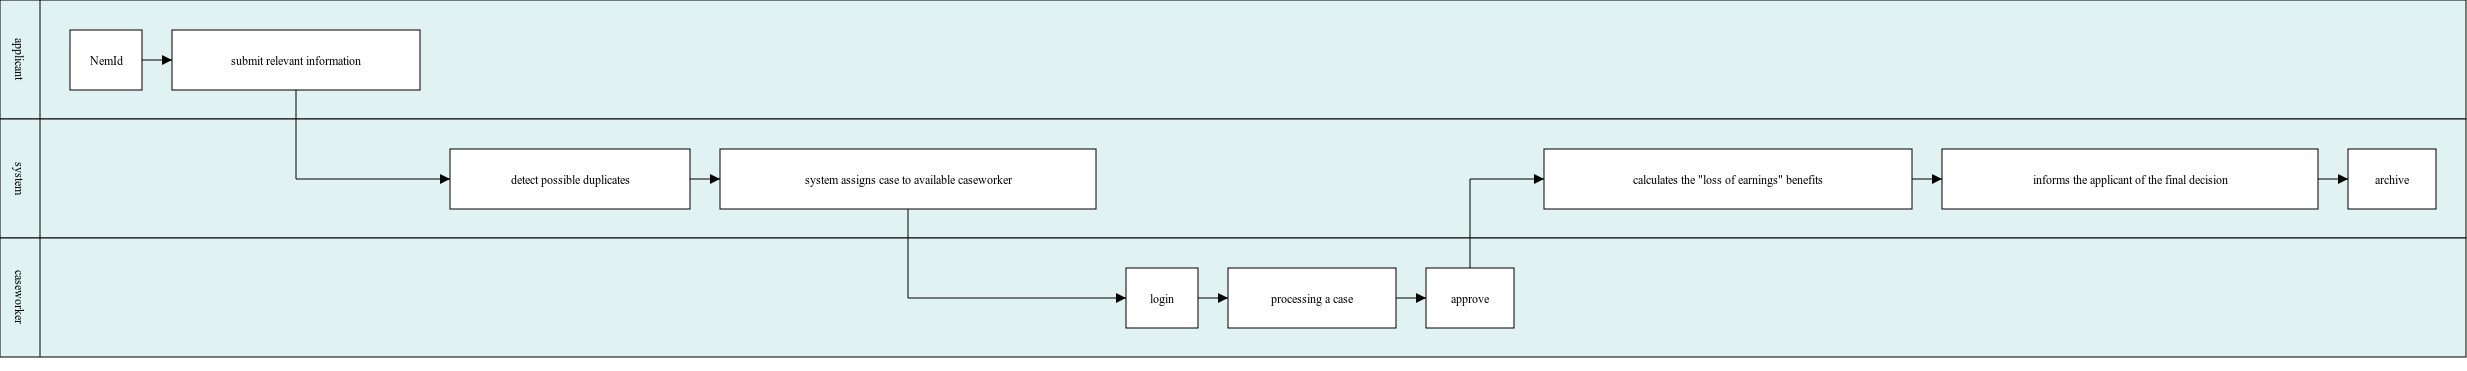
\includegraphics[width=\textwidth]{dcrgraph/case-approved.png}
    \caption{Scenario case approved}
\end{figure}

\begin{figure}[htb!]
    \centering
    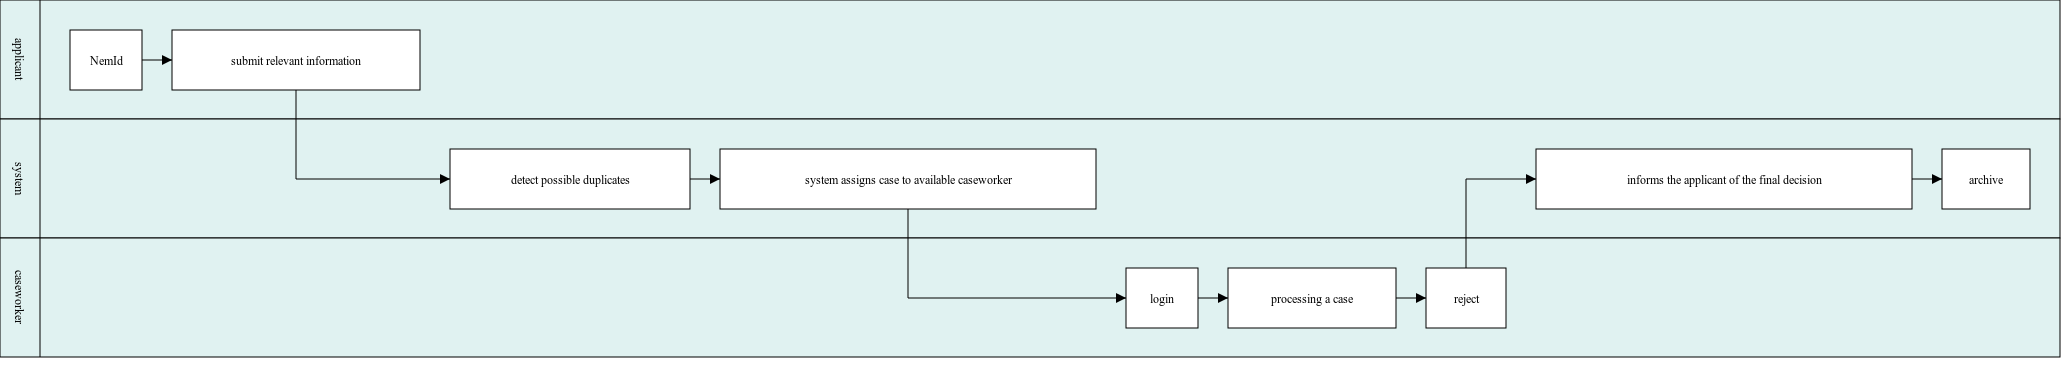
\includegraphics[width=\textwidth]{dcrgraph/case-rejected.png}
    \caption{Scenario case rejected}
\end{figure}

\begin{figure}[htb!]
    \centering
    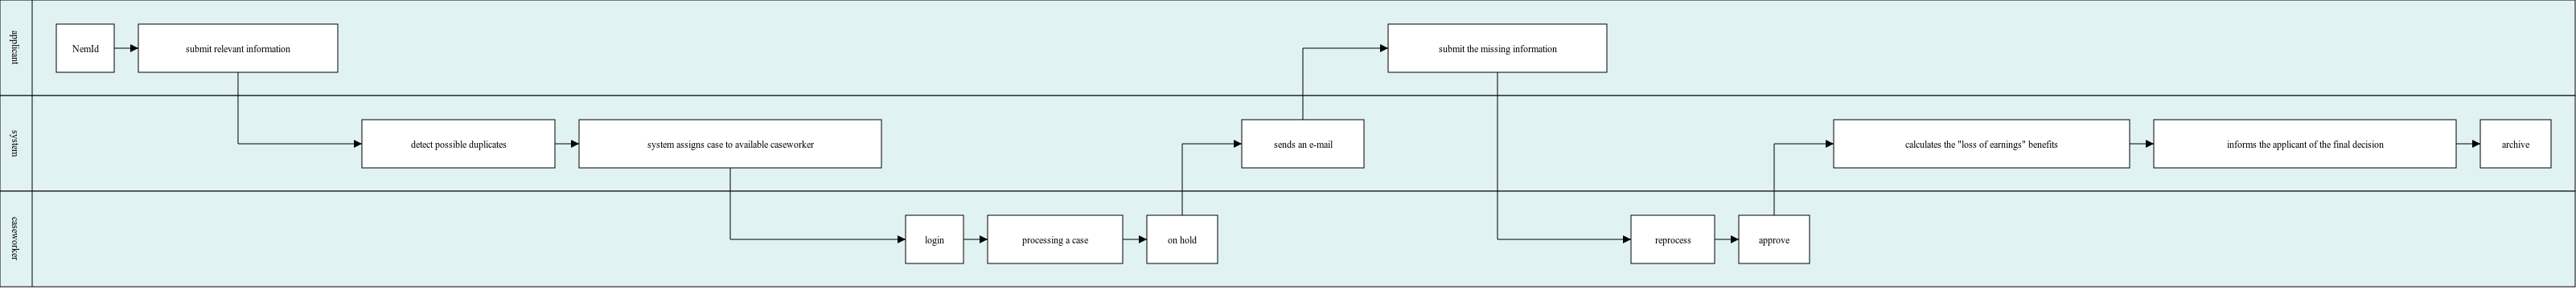
\includegraphics[width=\textwidth]{dcrgraph/case-inquire-information.png}
    \caption{Scenario inquire more information}
\end{figure}
